\item As shown in the figure, three identical polaroids \( P_1 \), \( P_2 \), and \( P_3 \) are placed one after another. The pass axis of \( P_2 \) and \( P_3 \) are inclined at angle of \( 60^\circ \) and \( 90^\circ \) with respect to axis of \( P_1 \). The source S has an intensity of \( 256 \frac{W}{m^2} \). The intensity of light at point O is \underline{\hspace{2.5cm}} \( \frac{W}{m^2} \). 
    
    \begin{center}
        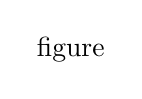
\begin{tikzpicture}
            \node at (0, 0) {{figure}};
        \end{tikzpicture}
    \end{center}